\subsection{Tensor Ring}


В работе \cite{DBLP:journals/corr/ZhaoZXZC16} исследуются свойства \textit{Tensor Ring Decomposition}, которое заключается в представлении тензора высокого порядка в виде последовательности трёхмерных тензоров, которые умножаются <<по кругу>>. Формально, пусть $\mathcal{T} \in \mathbb{R}^{n_1 \times n_2 \times \dotsm \times n_d}$ -- тензор высокого порядка, а $\mathcal{Z}_k \in \mathbb{R}^{r_k \times n_k \times r_{k + 1}}, k \in \overline{1, \dotsc, d}$ -- множество трёхмерных тензоров, такие что:

\begin{equation}\label{TRDecomp}
    \mathcal{T}(i_1, i_2, \dotsc, i_d) = \text{Tr}\{(\mathcal{Z}_1(i_1)\mathcal{Z}_2(i_2) \dotsm Z_d(i_d))\} = \text{Tr}\left\{\prod_{k=1}^d \mathcal{Z}_k(i_k)\right\},
\end{equation}

где $\mathcal{T}(i_1, i_2, \dotsc, i_d)$ -- число в многоиндексной таблице $\mathcal{T}$ с  индексами $i_1, i_2, \dotsc, i_d$, а  $\mathcal{Z}_k(i_k), \forall k \in \overline{1, \dotsc, d}$ -- срез трехмерного тензора $\mathcal{Z}_k$ с размерностью  $r_k \times r_{k + 1}$:

\begin{figure}[h!tp]
    \centering
    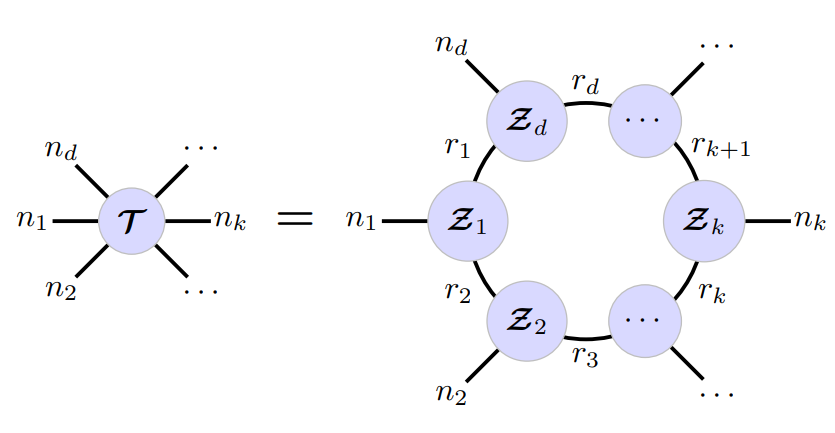
\includegraphics[scale=0.5]{TensorRing/DecompTR.PNG}
    \caption{Графическое представление \textit{Tensor Ring Decomposition}}
    \label{fig:TRDecomp}
\end{figure}


\textit{Tensor Ring Decomposition} в отличие от \textit{Tensor Train Decomposition} <<устойчиво>> по отношению к циклическим перестановкам рёбер тензора:


\textbf{Теорема}


Пусть $\mathcal{T} \in \mathbb{R}^{n_1 \times n_2 \times \dotsm \times n_d}$ -- тензор высокого порядка с \textit{Tensor Ring Decomposition} $\mathcal{R}(\mathcal{Z}_1, \mathcal{Z}_2, \dotsc, \mathcal{Z}_d)$. Определим тензор $\vec{\mathcal{T}} \in \mathbb{R}^{n_{k + 1} \times \dotsm \times n_d \times n_1 \times \dotsm \times n_k}$, полученный циклическим сдвигом рёбер исходного тензора $\mathcal{T}$ на $k$, тогда его \textit{Tensor Ring Decomposition} будет $\mathcal{R}(\mathcal{Z}_{k + 1}, \dotsc, \mathcal{Z}_d,  \mathcal{Z}_1, \dotsc, \mathcal{Z}_k)$

Также статья даёт ответы на вопросы о некоторых алгебраических свойствах разложения \textit{Tensor Ring} таких, как сложение и некоторые <<хитрые>> умножения.